\documentclass{ximera}

\title{Approximating Areas under Curves Facilitator Guide}
\author{MATH 425: Calculus I}

\begin{document}
\begin{abstract}
   Working with the peers in your group, solve the following problems. Make sure to show and justify all your work. Make sure everyone in the group understands the solution and participates. Be prepared to report your answers to the whole class. 
\end{abstract}
\maketitle

\textbf{Student Learning Outcomes}\\
Students should be able to: 
    \begin{itemize}
        \item Formulate and evaluate left-, right-, and midpoint-sums for a small number of rectangles and a given function and interval.
        \item Reason with the outputs of the sums.
        \item Use a simplified Riemann Sum definition of the integral to evaluate the exact area under a curve on an interval.
    \end{itemize}

\textbf{Prerequisite Knowledge:} Students should be familiar with the definitions of the three basic forms of Riemann sum: $L_n$, $R_n$, and $M_n$.  Students will also be expected to use and simplify sigma notation in problem (3) in order to use the Riemann sum definition to find an exact area.  

\begin{exercise}
    Consider the function $f(x)=3\sin(x)$ on the interval from $[0,\pi]$.  Estimate the area between $f(x)$ and the $x$-axis by \textit{formulating} $R_4$ and $L_4$.\\
    \textcolor{blue}{$R_4=(\frac{\pi}{4})3\sin(\frac{\pi}{4})+(\frac{\pi}{4})3\sin(\frac{\pi}{2})+(\frac{\pi}{4})3\sin(\frac{3\pi}{4})+(\frac{\pi}{4})3\sin(\pi)$\\%=\frac{3\pi\sqrt{2}}{8}+\frac{3\pi}{4}+\frac{3\pi\sqrt{2}}{8}+0=\frac{3\pi\sqrt{2}+3\pi}{4}$\\
    $L_4=(\frac{\pi}{4})3\sin(0)+(\frac{\pi}{4})3\sin(\frac{\pi}{4})+(\frac{\pi}{4})3\sin(\frac{\pi}{2})+(\frac{\pi}{4})3\sin(\frac{3\pi}{4})$\\}%=0+\frac{3\pi\sqrt{2}}{8}+\frac{3\pi}{4}+\frac{3\pi\sqrt{2}}{8}=\frac{3\pi\sqrt{2}+3\pi}{4}$}
    \textcolor{orange}{Note that ``formulate'' here means to set up but not evaluate the sum.  (The idea is to reinforce the concept without taking so long on tedious arithmetic.)}
\end{exercise}

\begin{exercise}
    Suppose that an object moving along a straight line path has its velocity in feet per second at time 
 in seconds given by $v(t)=\frac29(t-3)^2+2$.
 \begin{enumerate}
    \item Sketch the region whose exact area will tell you the distance the object travelled over the time interval $2\leq t\leq 5$.\\
    \begin{image}
        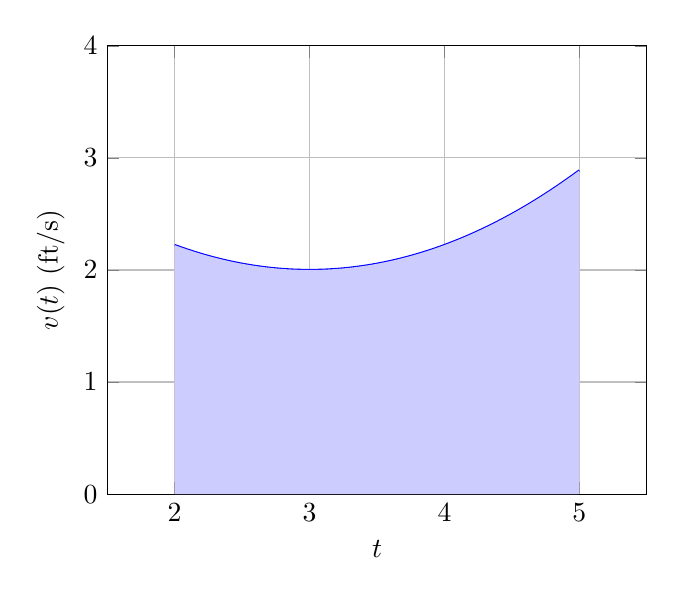
\begin{tikzpicture}
            \begin{axis}[
                xlabel=$t$,
                ylabel=$v(t)$ (ft/s),
                grid=major,
                domain=2:5,
                samples=100,
                xmin=1.5, xmax=5.5,
                ymin=0, ymax=4
            ]
            \addplot[blue, thick] {2/9*(x-3)^2 + 2};
            \addplot[draw=none, fill=blue!20] {2/9*(x-3)^2 + 2} \closedcycle;
            %\addplot[fill=blue!20, opacity=0.5] fill between[of=axis and plot1, soft clip={domain=2:5}];
            \end{axis}
        \end{tikzpicture}
    \end{image}
    %\xmalt{Sketch of the graph $y=\frac29(x-3)^2+2$ with the area between the curve and the $x$ axis from $t=2$ to $t=5$ shaded.}
    \item Estimate the distance travelled on $[2,5]$ by computing $L_3$, $M_3$, and $R_3$.\\
    \textcolor{blue}{$\Delta t=\frac{5-2}{3}=1$\\
    $L_3=v(2)(1)+v(3)(1)+v(4)(1)=(\frac29(1)+2)+(\frac29(0)+2)+(\frac29(1)+2)=\frac{58}{9}$\\
    $M_3=v(2.5)(1)+v(3.5)(1)+v(4.5)(1)=(\frac29(\frac14)+2)+(\frac29(\frac14)+2)+(\frac29(\frac94)+2)=6+\frac19+\frac12=\frac{119}{18}$\\
    $R_3=v(3)(1)+v(4)(1)+v(5)(1)=(\frac29(0)+2)+(\frac29(1)+2)+(\frac29(4)+2)=\frac{64}{9}$}
    \item Does averaging $L_3$ and $R_3$ result in the same value as $M_3$?  If not, what do you think the average of $L_3$ and $R_3$ measures?\\
    \textcolor{blue}{ $\frac{L_3+R_3}{2}=\frac{\frac{58}{9}+\frac{64}{9}}{2}=\frac{61}{9}(=\frac{122}{18})$\\
    The average of $L_3$ and $R_3$ is close to $M_3$, but not exactly equal.  The average is exactly halfway between $L_3$ and $R_3$, but $M_3$ will change based on the fact that the function is changing at different rates throughout the interval. This average would be exactly $M_3$ if the function was linear (same rate of change across the whole interval). }\\
    \textcolor{orange}{The reasoning part of this question is deeper than most students have probably gone with this content. It never hurts to ask students to sketch out the situation (with the rectangles) to reinforce their thinking. The hope is that the would notice that the midpoint (in the $x$-direction) is not always the midpoint in the $y$-direction.}
    \item or this question, think about an arbitrary function $f$, rather than the particular function $V$ given above. If $f$ is positive and increasing on $[a,b]$, will $L_n$ over-estimate or under-estimate the exact area under $f$ on $[a,b]$?  Will  $R_n$ over- or under-estimate the exact area under $f$ on $[a,b]$?Explain.\\
    \textcolor{blue}{If $f$ is positive and increasing, $L_n$ will be an underestimate because the lefthand side of the interval will always have a function value that is less than the value of the function on the rest of the interval.  If $f$ is increasing and positive, then $R_n$ is an overestimate because the righthand side of the interval will always have a function value that is greater than all the other values on the interval.  (If you're having trouble seeing or explaining this, try making a sketch.) }
 \end{enumerate}
Problem adapted from Boelkins, et al., \textit{Active Calculus}, 2nd ed. 

\end{exercise}

\begin{exercise}
    Use the following formulas to calculate the exact area under $g(x)=x^2-4x$ from $x=1$ to $x=3$.  $$\sum_{j=1}^{n} j=\frac{n(n+1)}{2}$$
    $$\sum_{j=1}^n j^2=\frac{n(n+1)(2n+1)}{6}$$\\
    \textcolor{blue}{For $n$ rectangles, $\Delta x=\frac{3-1}{n}$\\
    The endpoints will be $1, 1+\frac{2}{n}, 1+2(\frac{2}{n}), 1+3(\frac{2}{n}), ... 1+n(\frac{2}{n})$ or in general: $1+i(\frac{2}{n})$\\
    $\displaystyle R_n=\sum_{i=1}^n f(x_i)\Delta x=\sum_{i=1}^n \bigg((1+i(\frac{2}{n}))^2-4(1+i(\frac{2}{n})\bigg)(\frac{2}{n})$ \\
    $\displaystyle =\sum_{i=1}^n \bigg(1+2i(\frac{2}{n})+i^2(\frac{4}{n^2})-4-4i(\frac{2}{n})\bigg)(\frac{2}{n})$\\
    $\displaystyle =\sum_{i=1}^n \bigg(-3-2i(\frac{2}{n})+i^2(\frac{4}{n^2})\bigg)(\frac{2}{n})$\\
    $\displaystyle =\sum_{i=1}^n \bigg(3(\frac{2}{n})+2i(\frac{4}{n^2})+i^2(\frac{8}{n^3})\bigg)$\\
    $\displaystyle=\sum_{i=1}^n -3(\frac{2}{n})-\sum_{i=1}^n i(\frac{8}{n^2})+\sum_{i=1}^n i^2(\frac{8}{n^3}) $\\
    $\displaystyle=\sum_{i=1}^n \frac{-6}{n}-(\frac{8}{n^2})\sum_{i=1}^n i+(\frac{8}{n^3})\sum_{i=1}^n i^2 $\\
    $\displaystyle =\frac{-6}{n}(n)-\frac{8}{n^2}(\frac{n(n+1)}{2})+\frac{8}{n^3}(\frac{n(n+1)(2n+1)}{6})$\\
    $\displaystyle =-6-\frac{8(n+1)}{2n}+\frac{8(n+1)(2n+1)}{6n^2}$\\
    Then the area is the limit of $R_n$ as n goes to infinity:\\
    $\displaystyle\lim_{n\rightarrow \infty} R_n=\lim_{n\rightarrow \infty} \bigg( -6-\frac{4(n+1)}{n}+\frac{4(n+1)(2n+1)}{3n^2}\bigg)=-6-4+\frac{8}{3}=-\frac{22}{3}$\\}
    \textcolor{orange}{This problem is difficult for students, and this is likely to be the only time they work out a problem like this except for the presentation in lecture.  It may be worth going over this problem as a whole class, especially if groups are getting stuck.  }
\end{exercise}   

\end{document}